\chapter{Your figures and tables: a check of everything you have}
\label{ch:figures}

Figures are often the first thing a professor reads. This chapter checks every figure the project has, says which are correct, which need fixing and which should not be used, and lists the tables the report needs.

\section{Your professor's rules for figures and tables}

\begin{itemize}
  \item Figures and tables appear close to where they are first mentioned.
  \item Related panels are combined into one figure labelled (a), (b), (c).
  \item Text in figures must be legible after scaling (at least about 8\,pt); check by printing one page.
  \item Tables are real tables (\texttt{booktabs} in LaTeX), never screenshots of tables.
  \item The study-area map shows the whole of India, not trimmed at the top.
  \item Extra figures and tables go to an appendix.
\end{itemize}

\section{Every figure, checked}

\begin{longtable}{L{4.0cm}L{4.6cm}L{2.0cm}L{3.4cm}}
\caption{All figures in the project. ``Main'' = main text; ``App.'' = appendix.}\label{tab:figaudit}\\
\toprule
\textbf{File} & \textbf{What it shows} & \textbf{Status} & \textbf{Use} \\
\midrule
\endfirsthead
\toprule
\textbf{File} & \textbf{What it shows} & \textbf{Status} & \textbf{Use} \\
\midrule
\endhead
\file{papers/acl/fig_workflow.png} & your five-stage workflow & needs fixing & Main (Methods), after the fixes in Section~\ref{sec:fixworkflow} \\
\file{study_guide_v2/figures/fig_workflow_corrected.png} & the same figure with the fixes made & correct & Main, if you prefer it to fixing your own \\
\file{results/ecoexplain_vlm_pipeline.png} & an older pipeline drawing & outdated & Do not use: says ``LLaVA-1.5'', ``train on the train split'' and ``64\,$\times$\,64 pixels'' \\
\file{results/result1.png} & notebook flow 01--09 & outdated & Do not use: says ``LLaVA-1.5'' \\
\file{results/result2.png} & zero-shot results as an image of a table & wrong & Do not use: wrong encoder for LLaVA (``CLIP-ViT-L/14'', really SigLIP), and a table as an image \\
\file{results/explain/summary_scores.png} & early explanation-mode accuracy & outdated & Do not use: Qwen bars from 3 patches, before Phases C and D \\
\file{study_guide/figures/fig_patch_map.png} & candidate pool and selected patches by class and split & correct & Main (study area), next to an India map \\
\file{fig_ndvi_labels.png} & \dndvi{} distribution and the percentile rule & correct & Main (labelling) \\
\file{fig_label_vs_trend.png} & label against the card's trend words & correct & Main or App. \\
\file{fig_examples.png} & four test patches, colour pairs and \dndvi{} maps & correct & Main (dataset) \\
\file{fig_climate_by_class.png} & climate by class and year & correct & Main or App. \\
\file{fig_padding_bias.png} & the padding bias & correct & App. or Limitations \\
\file{fig_accuracy_overview.png} & classification runs with intervals & superseded & Use \file{fig_accuracy_v2.png} instead \\
\file{study_guide_v2/figures/fig_accuracy_v2.png} & classification runs up to 17 Oct & superseded & Use \file{fig_accuracy_v3.png} \\
\file{study_guide_v3/figures/fig_accuracy_v3.png} & every classification run, labelled by input, incl.\ the leak-free reruns & correct & Main (Track~A) or App. \\
\file{study_guide_v3/figures/fig_leakfree_confusion.png} & Qwen with and without the summary line; LLaVA with the compact table & correct & Main (Track~A): the key figure \\
\file{fig_confusion.png} & six confusion matrices & correct & Main: panels (a), (b); others App. \\
\file{study_guide_v2/figures/fig_lora_classes.png} & two LoRA runs (up to 17 Oct) & superseded & Use \file{fig_lora_v3.png} \\
\file{study_guide_v3/figures/fig_lora_v3.png} & training mix and test confusion of all three LoRA runs & correct & Main (fine-tuning) \\
\file{fig_explain_structured.png} & free-form against structured (Qwen, LLaVA) & superseded & Use \file{fig_explain_phases.png} \\
\file{study_guide_v2/figures/fig_explain_phases.png} & all explanation phases, four scores & correct & Main (explanations) \\
\file{fig_panel_p00575.png} & one patch, four models' free-form explanations & correct & App. (crop the empty space) \\
\file{fig_otsu_p01289.jpg} & Otsu boxes on one patch & pre-colour-fix & App. only, with a caption note \\
\textbf{study-area map of India} & --- & \textbf{missing} & Main: must be made (Section~\ref{sec:map}) \\
\bottomrule
\end{longtable}

\begin{watchout}
The per-model files in \file{results/protocol/} still label LLaVA ``LLaVA-1.5, CLIP-ViT-L/14''. If you plot from them, take the model name from Table~\ref{tab:models}, not from the file.

Figures saved under \file{study_guide/figures/}, \file{study_guide_v2/figures/} and \file{study_guide_v3/figures/} were made for learning. If you put one in the report, regenerate it (the scripts are \file{study_guide/make_figures.py} and \file{study_guide_v2/make_figures_v2.py}), check every label, and write your own caption. A figure in your report is your responsibility.
\end{watchout}

\section{Fixing your workflow figure}
\label{sec:fixworkflow}

Your figure (Figure~\ref{fig:workflow-yours}) is clear and well designed. Three box texts in stage~05 and two in stage~03 are inaccurate or vague, and two arrows are missing. Table~\ref{tab:workflowfix} lists the changes with the line numbers in \file{papers/acl/make_workflow_figure.py}.

\begin{longtable}{L{1.3cm}L{5.3cm}L{7.6cm}}
\caption{Changes to \file{make_workflow_figure.py}. A corrected copy is \file{study_guide_v2/make_workflow_figure_corrected.py} (every change is marked \texttt{CORRECTED} or \texttt{ADDED}).}\label{tab:workflowfix}\\
\toprule
\textbf{Line} & \textbf{Now} & \textbf{Change to, and why} \\
\midrule
\endfirsthead
\toprule
\textbf{Line} & \textbf{Now} & \textbf{Change to, and why} \\
\midrule
\endhead
219 & Track~A: ``Condition C: T0/T1 RGB + card / Qwen2-VL-2B $\cdot$ PaliGemma-3B / LLaVA-Interleave-0.5B $\cdot$ BLIP-2 / Full card and evidence\_only'' & ``Qwen2-VL-2B, LLaVA-0.5B: T0/T1 + full card / PaliGemma-3B: T0/T1 + NDVI line only / BLIP-2: stitched T0|T1, no card / evidence\_only: label line removed''. \emph{Why:} the four models did not receive the same input (Table~\ref{tab:inputs}). \\
230--231 & Track~B: ``(smoke test)'' and ``100\% run with leak is invalid'' & Title ``(16 patches, 1 epoch)''; body ``full card at train and test / first 16 training patches (9/6/1) / 256-patch runs reached 100\% by reading the label, so they are excluded''. \emph{Why:} the reported run should be described by its size, and the reason for excluding the 100\,\% runs is clearer than the word ``invalid''. \\
242--243 & Track~C: ``Free-form vs structured cite-only / Claims scored against the card / Optional 2B-on-2B explain LoRA'' & ``free-form prompt $\rightarrow$ structured cite-only prompt / claim directions checked against measured $\Delta$ / explanation LoRA pilot: 16 filtered 2B targets, all labelled decline''. \emph{Why:} claims are checked against the \emph{measured changes}, not ``the card''; and the explanation LoRA was run, so it is not ``optional''. \\
209 & ``05 Three evaluation tracks (do not mix the scores)'' & ``05 Three evaluation tracks (inputs differ: do not mix the scores)''. \emph{Why:} says why. \\
165, 176, 187 & stage~03 box texts & RGB chips: ``on a 512\,$\times$\,512 canvas; BLIP-2: one stitched image''. Label: give the cut-offs ``q15 = $-$0.038 $\cdot$ q85 = +0.003''. Card: ``last line repeats candidate\_class=''. \\
after 189 and 206 & arrows only through the middle column & add arrows from Earth Engine to the RGB and card boxes, and from those boxes to the split box: all three feed every record. \\
\bottomrule
\end{longtable}

\begin{figure}[H]
\centering
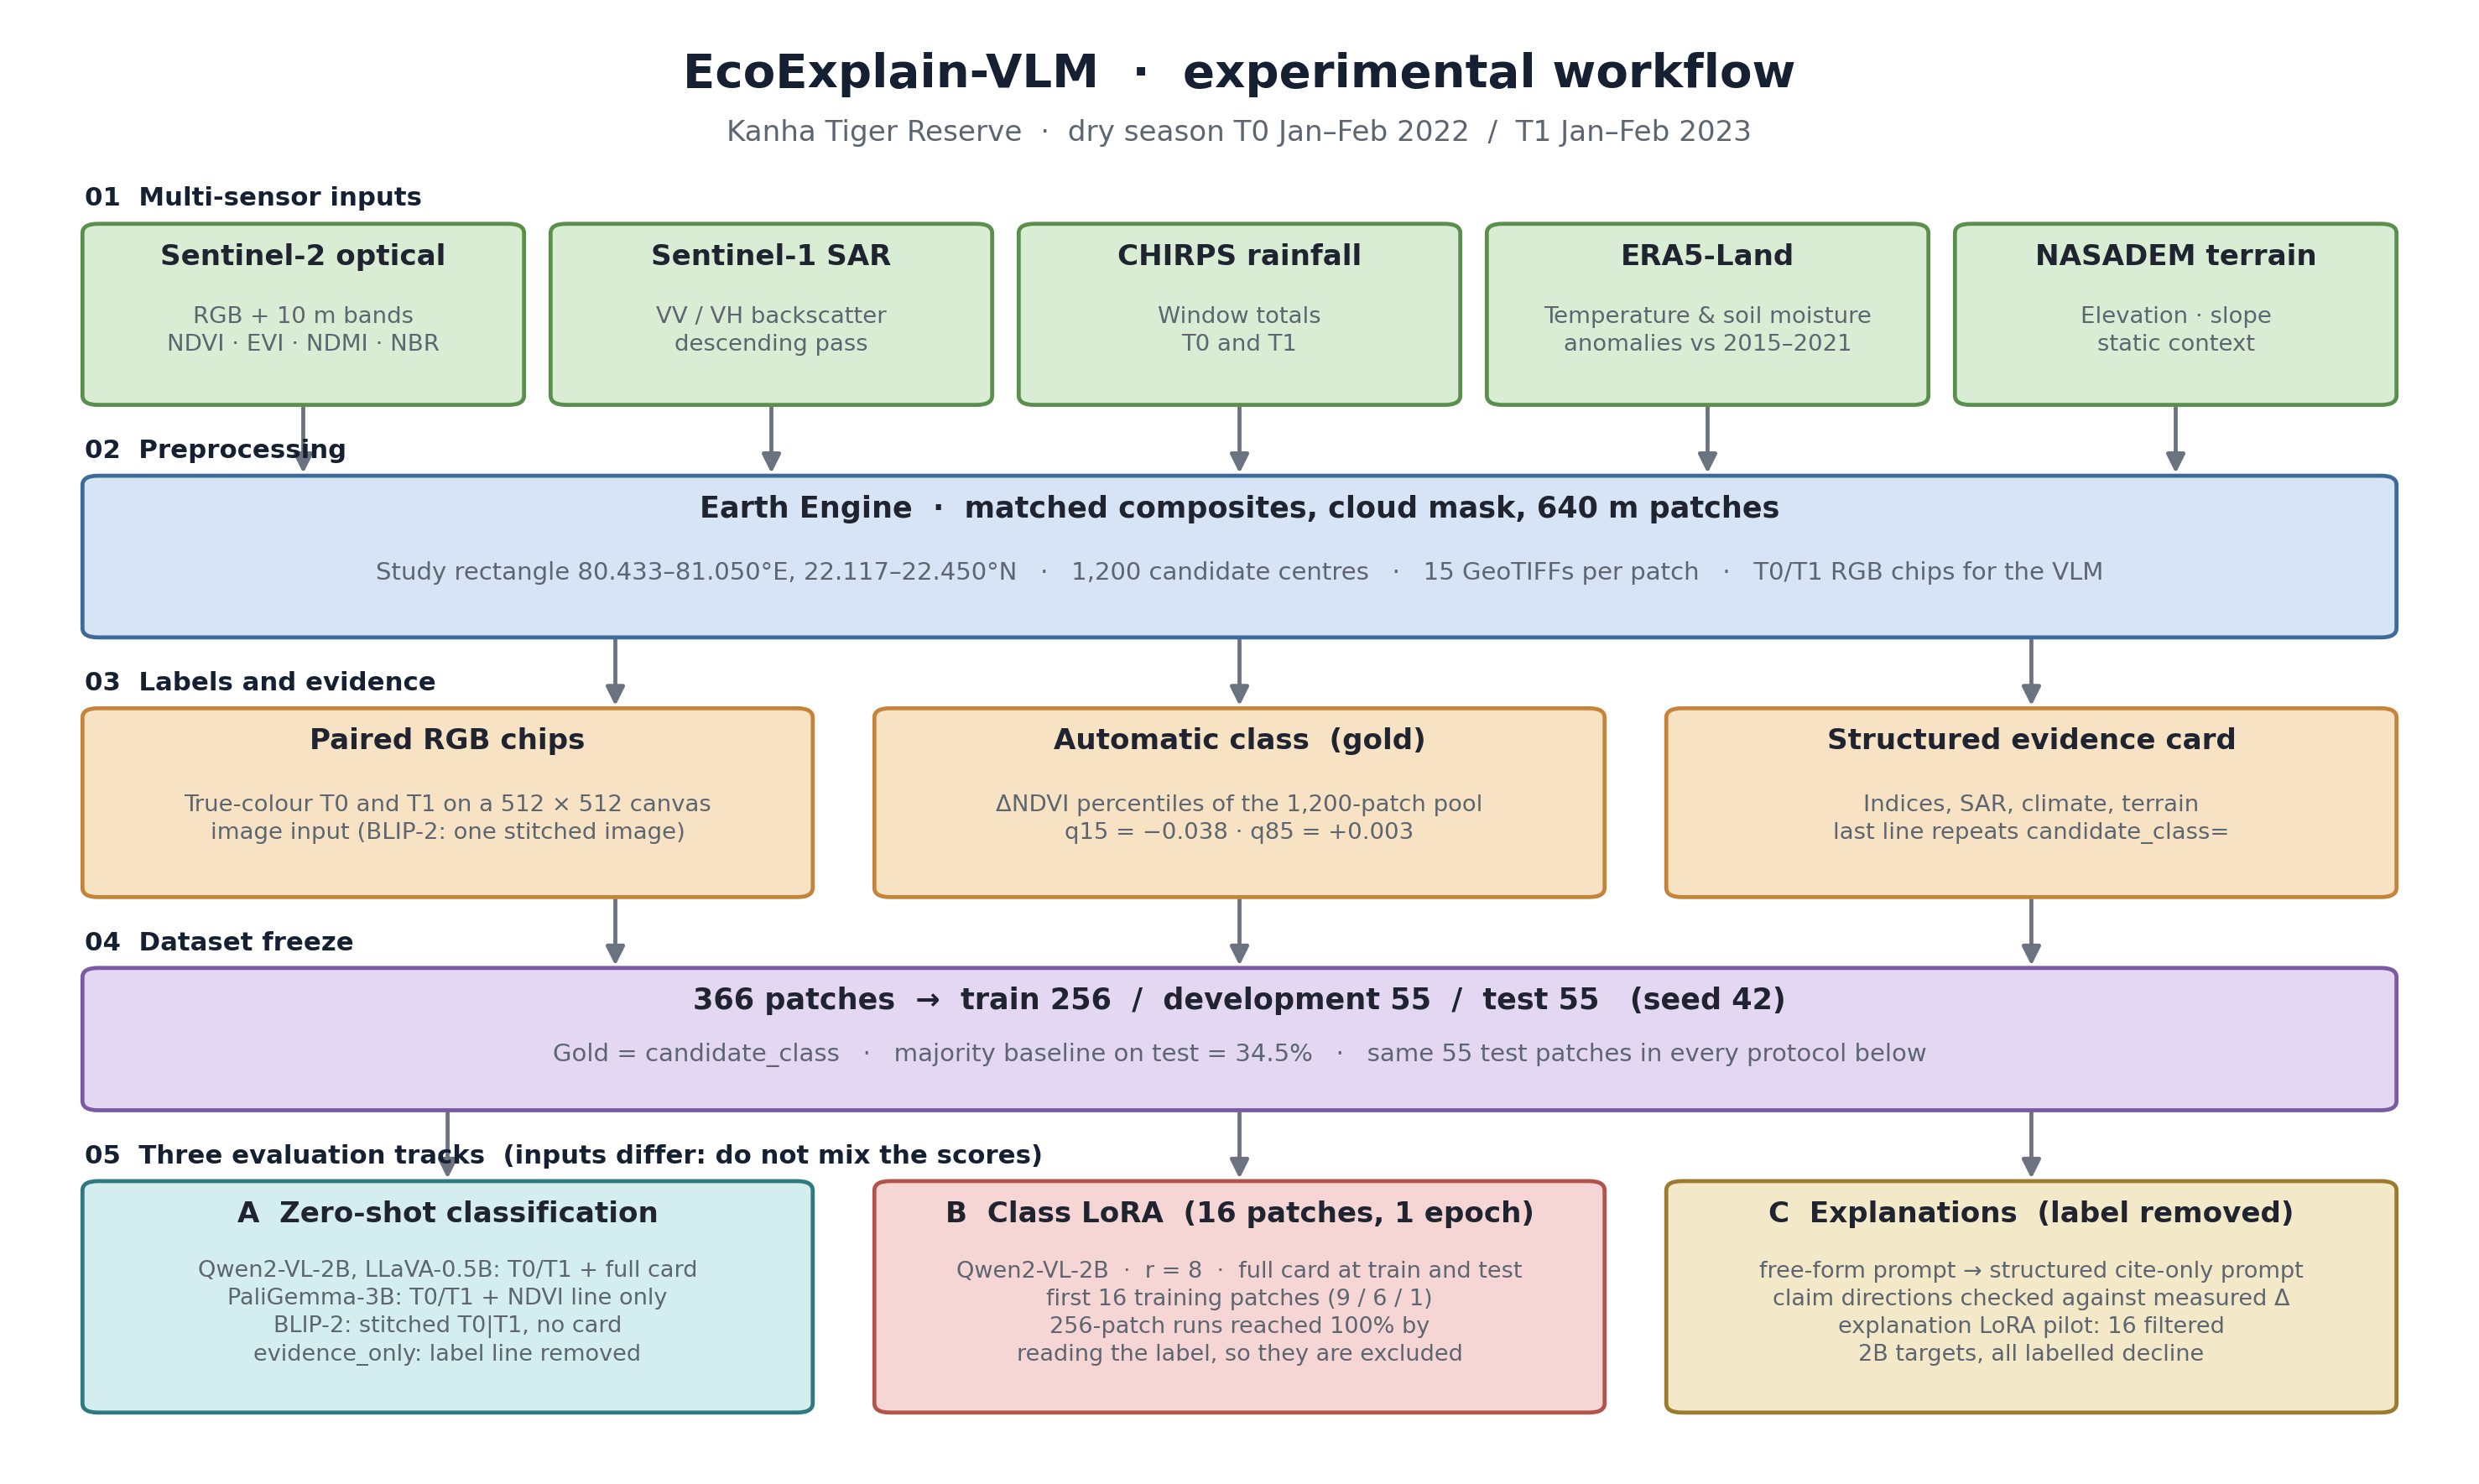
\includegraphics[width=\textwidth]{figures/fig_workflow_corrected.png}
\caption{Your workflow figure with the changes of Table~\ref{tab:workflowfix} (\file{study_guide_v2/make_workflow_figure_corrected.py}). Compare it box by box with Figure~\ref{fig:workflow-yours}.}
\label{fig:workflow-corrected}
\end{figure}

\begin{plainwords}
You can either edit your own script with the changes above (better: it stays your figure) or use the corrected copy. Either way, run it once more after any later change to the text of the report, so that the figure and the text say the same thing.
\end{plainwords}

\section{The study-area map}
\label{sec:map}

Your professor asks for a study-area map showing the whole of India without trimming at the top. You do not have one yet. A good layout has two or three panels:
\begin{enumerate}[label=(\alph*)]
  \item India with state boundaries and Madhya Pradesh highlighted. Use the official Survey of India boundary (from the Survey of India or the Bhuvan portal); maps of India in Indian academic work are expected to follow it, and many global boundary datasets do not.
  \item Madhya Pradesh with the reserve (for example, the boundary from the World Database on Protected Areas) and the study rectangle.
  \item The rectangle with the 366 patch points coloured by class (the content of Figure~\ref{fig:patchmap}).
\end{enumerate}
QGIS is the easiest tool; Python with \texttt{geopandas} and \texttt{matplotlib} also works. Add a north arrow, a scale bar and the coordinate grid.

\section{Tables the report needs}

\begin{table}[H]
\centering
\small
\begin{tabularx}{\textwidth}{lYl}
\toprule
Table & Content & Based on \\
\midrule
Data sources & collection, variables, resolution, scenes & Table~\ref{tab:sources} \\
Dataset summary & patches, classes, split, baseline, human agreement & Table~\ref{tab:split} and Chapter~\ref{ch:stage03} \\
Model inputs & what each model received & Table~\ref{tab:inputs} \\
Classification results & accuracy, interval, macro-F1, input & Table~\ref{tab:trackA}; baselines from Chapter~\ref{ch:trackA} \\
LoRA configuration & settings of both runs & Table~\ref{tab:classlora} \\
Fine-tuning jobs (App.) & all Ada jobs & Table~\ref{tab:ftruns} \\
Explanation results & Phases B, C, D & Tables~\ref{tab:phaseB}--\ref{tab:phaseD} (shortened) \\
\bottomrule
\end{tabularx}
\end{table}

\begin{foryourreport}
Your current draft (ACL two-column format) has one figure. A report of 8,500--10,000 words can carry about six to eight figures in the main text: the study-area map, the workflow, the \dndvi{} labelling figure, the example patches, the classification results, the LoRA confusion matrices, and the explanation summary. In two-column format, use \texttt{figure*} for wide figures (workflow, examples) and \texttt{figure} with \texttt{width=\textbackslash columnwidth} for narrow ones.
\end{foryourreport}

\begin{selfcheck}
\begin{enumerate}
  \item Which existing figures should not appear in the report, and why?
  \item What exactly is wrong with Track~A in your workflow figure?
  \item What must the study-area map show, according to your professor?
\end{enumerate}
\end{selfcheck}
